%% =============================================================================
%% ОБЩИЕ ПРАВИЛА (для людей и для ИИ-агентов)
%% =============================================================================
%% 1. Это черновик ОДНОГО участника. Редактируй только этот файл.
%% 2. Не меняй чужие файлы в папке drafts/.
%% 3. Не трогай корневой main.tex, преамбулу, стили (.cls, .sty), .github/.
%% 4. Можно использовать существующие метки (
ef, \label, \cite), но не переименовывай их без согласования.
%% 5. Новые рисунки складывай в figures/ с уникальным именем: <имя>_<смысл>.png.
%% 6. Новые источники (BibTeX) пришли Давиду (david_final.tex) или в issues.
%% 7. Сохраняй статью в формате IEEEtran; не меняй шрифты/поля.
%% 8. После правки скинь файл координатору; сборка PDF делается в main.tex.
%% =============================================================================

%% УЧАСТНИК: Глеб
%% РАЗДЕЛЫ: Introduction + History and background: from SCADA to AI-aided control systems
%% ЗАДАЧИ:
%%   - Переписать Abstract и keywords (они ниже в david_final.tex, но Глеб предлагает версию в комментарии/issue).
%%   - Сделать Introduction заточенной под пастеризационную установку.
%%   - Сократить/переформулировать историю SCADA, убрать длинные списки.
%%   - Обновить рисунок "Neural Network as a Black Box" (figures/ или TikZ).
%%   - Добавить 2-3 свежих источника по SCADA + AI.
%% =============================================================================

\section{Introduction}

This paper builds upon the ideas discussed in
\cite{ivaniuk2025neurosymbolic,ivaniuk2024neurosemantic,Lutska2022,Taberko2020,
Golovko2018integration} and reviews current challenges and tools for developing
and applying industrial standards alongside modern techniques such as
neuro-control, \textbf{neuro-symbolic AI}, and semantic technologies. It also
summarizes the history of \textbf{SCADA} systems and their evolution into modern
control systems integrated with AI and Industry 4.0 technologies. The main focus
is on standards-related problems and their relevance to today's control systems.
A symbolic neurocontroller is presented as a promising approach for controlling
complex industrial processes such as pasteurization by combining the strengths
of symbolic and neural methods. Each level is governed by its own algorithms and
often resembles a black box: inputs and outputs are visible, while the internal
algorithm is hidden. For instance, a neural network can be represented as a
black box (Fig.~\ref{fig:black_nn}), but it remains important to understand the
underlying rules.

\begin{figure}[ht]
  \centering
  \begin{adjustbox}{width = \columnwidth}
    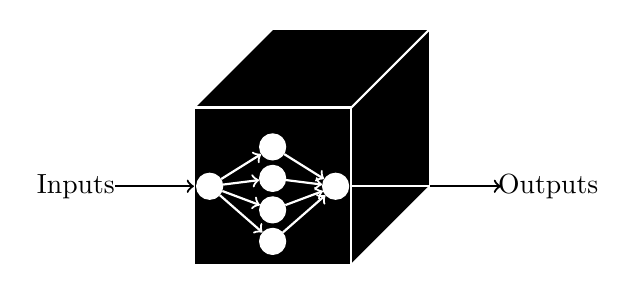
\begin{tikzpicture}


      % Draw the black box.
      \fill[black] (0,0) -- (2,0) -- (2,2) -- (0,2) -- cycle; % Front
      \fill[black] (2,0) -- (3,1) -- (3,3) -- (2,2);          % Right
      \fill[black] (0,2) -- (1,3) -- (3,3) -- (2,2) -- cycle; % Top

      % Draw the edges of the black box.
      \draw[thick, white] (0,0) -- (2,0) -- (2,2) -- (0,2) -- cycle; % Front
      \draw[thick, white] (2,0) -- (3,1) -- (3,3) -- (2,2);          % Right
      \draw[thick, white] (0,2) -- (1,3) -- (3,3);                   % Top

      % Draw a simple neural network on the front surface of the box.
      \node[draw=white, fill=white, circle] (in) at (0.2,1) {};
      \node[draw=white, fill=white, circle] (h1) at (1,1.5) {};
      \node[draw=white, fill=white, circle] (h2) at (1,1.1) {};
      \node[draw=white, fill=white, circle] (h3) at (1,0.7) {};
      \node[draw=white, fill=white, circle] (h4) at (1,0.3) {};
      \node[draw=white, fill=white, circle] (out) at (1.8,1) {};

      \draw[white, thick, ->] (in) -- (h1); \draw[white, thick, ->] (in) --
      (h2); \draw[white, thick, ->] (in) -- (h3); \draw[white, thick, ->] (in)
      -- (h4); \draw[white, thick, ->] (h1) -- (out); \draw[white, thick, ->]
      (h2) -- (out); \draw[white, thick, ->] (h3) -- (out); \draw[white, thick,
      ->] (h4) -- (out);

      % Draw the input arrow and text.
      \draw[thick, ->] (-1,1) -- (0,1); \node at (-1.5,1) {Inputs};

      % Draw the output arrow and text.
      \draw[thick, ->] (3,1) -- (3.9,1); \draw[white, thick, -] (2,1) -- (3,1);
      \node at (4.5,1) {Outputs};
    \end{tikzpicture}
  \end{adjustbox}

  \caption{Neural Network as a Black Box}
  \label{fig:black_nn}
\end{figure}

\section{History and background: from \texorpdfstring{\textbf{SCADA}}{SCADA} to
\texorpdfstring{\textbf{AI-aided control systems}}{AI-aided control systems}}

Supervisory Control and Data Acquisition (\textbf{SCADA}) systems have become
the backbone of modern industrial automation and control infrastructure. From
power generation and distribution to water treatment, oil and gas pipelines, and
manufacturing facilities, \textbf{SCADA} systems enable centralized monitoring
and control of geographically distributed processes.

Let us examine the evolution of \textbf{SCADA} systems over the past six decades
\cite{boyer2004scada,MFGTechHub2024,TechTarget2024}, tracing their development
from simple telemetry systems to sophisticated, networked control platforms.
Understanding this historical progression is essential for appreciating current
\textbf{SCADA} capabilities and anticipating future trends in industrial
automation.

The rapid pace of technological change in industrial control systems
necessitates a historical perspective to understand how \textbf{SCADA} systems
evolved to meet changing industrial needs, regulatory requirements, and
cybersecurity challenges.

\subsection{Pre-\textbf{SCADA} Era (Before 1960s)} Before the advent of
\textbf{SCADA} systems, industrial processes relied on manual monitoring and
control. Operators physically inspected equipment, read gauges, and manually
adjusted controls. This approach was labor-intensive, prone to human error, and
limited to small-scale operations.

\subsection{Birth of \textbf{SCADA} (1960s-1970s)} The first generation of
\textbf{SCADA} systems emerged in the 1960s as mainframe-based monolithic
systems. These early systems were characterized by:

\begin{itemize}
    \item \textbf{Centralized Architecture}: All processing occurred at a
    central mainframe computer
    \item \textbf{Proprietary Protocols}: Vendor-specific communication
    protocols with no standardization
    \item \textbf{Relay Logic}: Control based on relay circuits and hard-wired
    logic
    \item \textbf{Limited Connectivity}: Point-to-point connections using serial
    communication
    \item \textbf{Basic Telemetry}: Simple Remote Terminal Units for data
    collection
\end{itemize}

Several factors drove the development of early \textbf{SCADA} systems (Key
Drivers):
\begin{enumerate}
    \item Need for remote monitoring of geographically dispersed infrastructure
    \item Labor cost reduction through automation
    \item Improved safety through continuous monitoring
    \item Enhanced operational efficiency and response times
\end{enumerate}

\subsection{Second Generation: Distributed \textbf{SCADA} (1970s-1980s)} The
second generation introduced distributed computing concepts. Multiple computers
were networked using Local Area Networks (LANs), sharing control and monitoring
responsibilities. Key characteristics included:

\begin{itemize}
    \item Multiple systems performing similar functions
    \item Introduction of minicomputers
    \item LAN-based communication between systems
    \item Still largely proprietary protocols
    \item Improved redundancy and reliability
\end{itemize}

\subsection{Third Generation: Networked \textbf{SCADA} (1990s-2000s)} The third
generation marked a significant shift toward open systems and standard
protocols:

\begin{itemize}
    \item \textbf{Open Architecture}: Adoption of industry standards (e.g.,
    TCP/IP, Ethernet)
    \item \textbf{Standard Protocols}: Implementation of protocols like Modbus,
    DNP3, IEC 60870-5-104
    \item \textbf{Client-Server Model}: Separation of data acquisition and
    presentation layers
    \item \textbf{WAN Connectivity}: Wide Area Network communication enabled
    \item \textbf{COTS Components}: Use of Commercial Off-The-Shelf hardware and
    software
    \item \textbf{Human-Machine Interface (HMI)}: Advanced graphical user
    interfaces
\end{itemize}

\subsection{Fourth Generation: Internet of Things \textbf{SCADA}
(2010s-Present)} Modern \textbf{SCADA} systems integrate IoT technologies and
cloud computing:

\begin{itemize}
    \item Cloud-based \textbf{SCADA} platforms
    \item Big data analytics and machine learning integration
    \item Mobile device support for remote access
    \item Enhanced cybersecurity measures
    \item Edge computing capabilities
    \item Integration with Enterprise Resource Planning (ERP) systems
    \item Real-time data analytics and predictive maintenance
\end{itemize}


The evolution of SCADA has been closely tied to advances in communication
technology and hardware capabilities. As communication technologies evolved,
SCADA systems were able to expand their reach and functionality. The following
tables summarize the key communication technologies that have shaped SCADA
development over the years:

\begin{table}[h]
\centering
\caption{Evolution of SCADA Communication Technologies}
\label{tab:communication}
\begin{tabular}{@{}lll@{}} \textbf{Era} & \textbf{Technology} &
\textbf{Characteristics} \\
1960s--1970s & Serial/Analog Radio & Point-to-point, low bandwidth \\
1980s--1990s & Digital Radio & Improved reliability, bandwidth \\
1990s--2000s & Ethernet, TCP/IP & Standard protocols, LAN/WAN \\
2000s--2010s & Wireless, Cellular & Mobile connectivity, flexibility \\
2010s--Present & IoT, 5G, Satellite & High bandwidth, global coverage \\
\end{tabular}
\end{table}

\begin{table}[h]
  \centering
  \caption{Hardware evolution of SCADA systems}
  \label{tab:hardware_evolution}
  \begin{tabular}{@{}ll@{}} \textbf{Era} & \textbf{Key hardware} \\
    1960s--1970s & Mainframes, relay logic, basic RTUs \\
    1980s--1990s & Minicomputers, Programmable Logic Controllers (PLCs) \\
    1990s--2000s & Industrial PCs, advanced RTUs with local intelligence \\
    2000s--Present & Edge devices, IoT sensors, distributed processing units \\
  \end{tabular}
\end{table}

Software has been crucial to SCADA evolution:
\begin{itemize}
    \item Early proprietary software systems
    \item Introduction of databases for historical data storage
    \item Development of sophisticated HMI/SCADA software packages
    \item Web-based interfaces and mobile applications
    \item Integration with data analytics and AI platforms
\end{itemize}

Key protocols that shaped SCADA development include:
\begin{itemize}
    \item \textbf{Modbus} (1979): Simple master-slave protocol, still widely
    used
    \item \textbf{DNP3} (1993): Developed for electric utilities, robust and
    efficient
    \item \textbf{IEC 60870-5-104} (2000): International standard for power
    system control
    \item \textbf{OPC} (1996): Standardized data exchange between industrial
    systems
    \item \textbf{MQTT} (1999): Lightweight publish-subscribe protocol for IoT
    \item \textbf{OPC UA} (2006): OPC Unified Architecture
\end{itemize}

Modern SCADA systems are integral to the Fourth Industrial Revolution (Industry
4.0), characterized by:
\begin{itemize}
    \item Cyber-physical systems integration
    \item Internet of Things (IoT) connectivity
    \item Cloud computing and edge processing
    \item Big data analytics and artificial intelligence
    \item Digital twins for simulation and optimization
    \item Augmented reality for maintenance and training
    \item Cloud SCADA platforms
\end{itemize}

However, they also introduce concerns about data security, latency, and
reliability.

Modern SCADA systems leverage advanced analytics:
\begin{itemize}
    \item Predictive maintenance using machine learning algorithms
    \item Anomaly detection for early fault identification
    \item Process optimization through data-driven insights
    \item Energy consumption analysis and optimization
    \item Quality control through statistical process control
\end{itemize}

Despite standardization efforts, challenges remain: legacy systems using
proprietary protocols, integration of diverse vendor equipment, need for gateway
devices and protocol converters and ongoing standardization efforts (e.g., OPC
UA).

Many organizations face challenges in upgrading aging SCADA infrastructure:
\begin{itemize}
    \item High costs of replacement
    \item Risk of operational disruption
    \item Limited support for obsolete components
    \item Need for phased migration strategies
\end{itemize}

Several trends are shaping the future of SCADA:
\begin{itemize}
    \item \textbf{Edge Computing}: Processing data closer to sources for reduced
    latency
    \item \textbf{5G Networks}: Enabling real-time control over wireless
    networks
    \item \textbf{Blockchain}: For secure data exchange and audit trails
    \item \textbf{Digital Twins}: Virtual replicas for simulation and
    optimization
    \item \textbf{AI-Driven Automation}: Autonomous decision-making systems
    \item \textbf{Quantum Computing}: Potential for complex optimization
    problems
\end{itemize}


